\documentclass[handout]{beamer}

\usetheme[progressbar=frametitle]{metropolis}
\usepackage{appendixnumberbeamer}
\usepackage{booktabs}
\usepackage{amsmath}
\usepackage{amssymb}
\usepackage{tcolorbox}
\usepackage{pgfplots}
% compatibility of pgfplots
\pgfplotsset{compat=1.16}
\usepackage{tikz}
\usepackage{pgf}
\definecolor{metropolisblue}{RGB}{39, 59, 94}



% Begin document
\begin{document}

% Title page
\title{Information Theory for Machine Learning}
\author{Nipun Batra}
\date{\today}
\institute{IIT Gandhinagar}
\maketitle


\begin{frame}{The Data Compression Problem}
    % Draw a TikZ figure showing the message, the source, the encoder, the message, the decoder, and the reconstructed message.
    \begin{figure}[h]
        \centering
        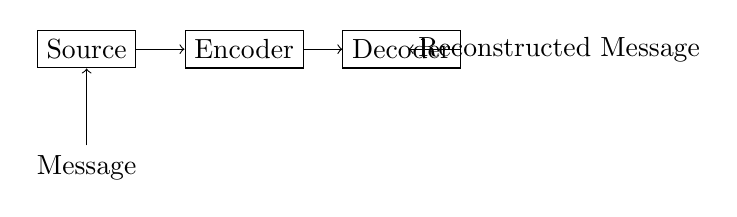
\begin{tikzpicture}[node distance=2cm,auto]
          % Nodes
          \node[draw, rectangle] (source) {Source};
          \node[below of=source, node distance=1.5cm] (message) {Message};
          \node[draw, rectangle, right of=source] (encoder) {Encoder};
          \node[draw, rectangle, right of=encoder] (decoder) {Decoder};
          \node[right of=decoder] (reconstructed) {Reconstructed Message};
      
          % Arrows
          \draw[->] (message) -- (source);
          \draw[->] (source) -- (encoder);
          \draw[->] (encoder) -- (decoder);
          \draw[->] (decoder) -- (reconstructed);
        \end{tikzpicture}
        \caption{Data Compression Problem}
      \end{figure}
    
\end{frame}


\begin{frame}{Self Information}
\begin{itemize}
    \item What is more surprising: Snowing in Kashmir or Snowing in Gandhinagar?
    \item To formalize, let us assume that the probability of snowing in Kashmir is $p_1$ and that in Gandhinagar is $p_2$, and that $p_1 >> p_2$.
    \item How can we quantify the surprise?
\end{itemize}
\end{frame}

\begin{frame}{Self Information}
    \begin{itemize}
        \item Events that are less likely to occur are more surprising.
        \item Also, if an event is 100\% likely to occur, it is not surprising at all.
        \item Also, if two events are independent, then the surprise of both of them occurring together is the sum of the surprise of each of them occurring individually.
        \item So, we need a function that maps probability to a number. Function  should be: monotonic, and additive, and is 0 when the probability is 1.
        \item The function is $I(x) = -\log_2(x)$ also called the self information or surprisal.
    \end{itemize}
    \end{frame}

\begin{frame}{Self Information}
    \begin{figure}
        \centering
        \includegraphics[width=0.8\textwidth]{notebooks/figures/information-theory/self-information.pdf}
        \caption{Self Information}
        \label{fig:self_info}
    \end{figure}
\end{frame}

\begin{frame}{Self Information}
    Consider a categorical random variable $X$ with $4$ possible outcomes: A, B, C, D. The probability of each of these outcomes is $0.25$. What is the self information of each of these outcomes?
    \begin{figure}
        \centering
        \includegraphics[width=0.8\textwidth]{notebooks/figures/information-theory/categorical-uniform.pdf}
        \label{fig:self_info_categorical_uniform}
    \end{figure}

    $I(A) = I(B) = I(C) = I(D) = 2$ bits.

\end{frame}

\begin{frame}{Self Information}
    Consider a categorical random variable $X$ with $4$ possible outcomes: A, B, C, D. The probability these outcomes is $0.5$, $0.25$, $0.125$, and $0.125$. What is the self information of each of these outcomes?
    \begin{figure}
        \centering
        \includegraphics[width=0.8\textwidth]{notebooks/figures/information-theory/categorical-nonuniform.pdf}
        \label{fig:self_info_categorical_nonuniform}
    \end{figure}

    $I(A) = 1$ bit, $I(B) = 2$ bits, $I(C) = I(D) = 3$ bits.

\end{frame}

\begin{frame}{Self Information}
    Proof on additivity of self information:
    Consider two independent random variables $X$ and $Y$ with PMFs $p_X(x)$ and $p_Y(y)$ respectively. The joint PMF is $p_{X, Y}(x, y) = p_X(x)p_Y(y)$. The self information of the joint PMF is:
    \begin{align*}
        I(X=x, Y=y)=& -\log_2(p_X(x)p_Y(y)) \\
        &= -\log_2(p_X(x)) - \log_2(p_Y(y))\\ &= I(X=x) + I(Y=y)
    \end{align*}
    
\end{frame}

\begin{frame}{Entropy}
    \begin{itemize}
        \item The entropy of a random variable is the expected value of the self information.
        \item $H(X) = \mathbb{E}_{X \sim p(x)}[I(X)] = \mathbb{E}_{X \sim p(x)}[-\log_2(p(x))]$
        \item The entropy of a random variable is the expected number of bits required to encode the random variable.
        \item The entropy of a random variable is the minimum number of bits required to encode the random variable.
    \end{itemize}
    
\end{frame}

\begin{frame}{Entropy}
    For a Bernoulli random variable $X$ with probability $p$ of success, the entropy is:
    \begin{align*}
        H(X) &= \mathbb{E}_{X \sim p(x)}[-\log_2(p(x))] \\
        &= -\log_2(p) \times p - \log_2(1-p) \times (1-p) \\
        &= -p\log_2(p) - (1-p)\log_2(1-p)
    \end{align*}
    \begin{figure}
        \centering
        \includegraphics[width=0.8\textwidth]{notebooks/figures/information-theory/entropy-bernoulli.pdf}
        \caption{Entropy}
        \label{fig:entropy}
    \end{figure}
    
\end{frame}

\begin{frame}{Entropy}
    For a $k$ class categorical random variable $X$ with probability $p_i$ of class $i$, the entropy is:
    \begin{align*}
        H(X) &= \mathbb{E}_{X \sim p(x)}[-\log_2(p(x))] \\
        &= -\sum_{i=1}^k p_i \log_2(p_i)
    \end{align*}

    \begin{figure}
        \centering
        \includegraphics[width=0.8\textwidth]{notebooks/figures/information-theory/categorical-entropy.pdf}
        \caption{Entropy}
        \label{fig:entropy_categorical}
    \end{figure}
    
\end{frame}

\begin{frame}{Code Length}
Let us assume our symbols are: A, B, C, D. Let us assume that the probability of each of these symbols is $0.25$. 
Let us assume we use the following code to encode these symbols:
\begin{align*}
    A &\rightarrow 00 \\
    B &\rightarrow 01 \\
    C &\rightarrow 10 \\
    D &\rightarrow 11
\end{align*}
What is the expected code length?

Expected code length = $L(X) = \sum_{i=1}^4 p_i \times l_i = 2$ bits.
    
\end{frame}

\begin{frame}{Code Length}
    Let us assume our symbols are: A, B, C, D. Let us assume that the probability of these symbols is $0.5$, $0.25$, $0.125$, and $0.125$. 
    Let us assume we use the following code to encode these symbols:
    \begin{align*}
        A &\rightarrow 00 \\
        B &\rightarrow 01 \\
        C &\rightarrow 10 \\
        D &\rightarrow 11
    \end{align*}
    What is the expected code length?
    
    Expected code length = $\sum_{i=1}^4 p_i \times l_i = 2$ bits.
    But, is this the most efficient code?
    \pause No! What is the entropy of this random variable?
    \pause $H(X) = 1.75$ bits.
        
    \end{frame}

    \begin{frame}{Code Length}
        Let us assume our symbols are: A, B, C, D. Let us assume that the probability of these symbols is $0.5$, $0.25$, $0.125$, and $0.125$. 
        Using fixed length codes, we need $2$ bits to encode each symbol.

        Key idea: Use shorter codes for more frequent symbols and longer codes for less frequent symbols.

        How about the following code?
        \begin{align*}
            A &\rightarrow 0 \\
            B &\rightarrow 10 \\
            C &\rightarrow 110 \\
            D &\rightarrow 111
        \end{align*}

        Expected code length = $\sum_{i=1}^4 p_i \times l_i = 1.75$ bits.
        
    \end{frame}

    \begin{frame}{Optimum Code Length}
        By definition, we saw that the entropy of a random variable is the minimum number of bits required to encode the random variable.

        This means that the expected code length of any code is always greater than or equal to the entropy of the random variable.
        \begin{tcolorbox}[colback=metropolisblue!5,colframe=metropolisblue,title={Relationship between entropy and expected code length}]
        \begin{equation}
            L(X) = \sum_{i=1}^n p_i \times l_i \geq H(X)
        \end{equation}
        \end{tcolorbox}

        Optimum length for each symbol is given by:
        \begin{equation}
            l_i = -\log_2(p_i)
        \end{equation}
        
    \end{frame}

    \begin{frame}{Huffman Encoding}
        \begin{itemize}
            \item Huffman encoding is a method to construct a variable length code for a random variable.
            \item The code is constructed such that the expected code length is equal to the entropy of the random variable.
            \item The code is constructed such that the code is a prefix code.
        \end{itemize}
        
    \end{frame}

    \begin{frame}{Cross Entropy}
        Suppose we have four symbols A, B, C, D with probabilities $0.5$, $0.25$, $0.125$, and $0.125$ respectively. Let us call this distribution $p(x)$.
        We want to transmit some data using these symbols. 

        The optimum encoding scheme is:
        A: 0, B: 10, C: 110, D: 111.
            
        \pause But, for some reason, we believe that the four symbols are distributed as per $q(x)$: $0.25$, $0.25$, $0.25$, and $0.25$. 
        
        For this distribution, the optimum encoding scheme is:
        A: 00, B: 01, C: 10, D: 11.

    \end{frame}
        
    \begin{frame}{Cross Entropy}
        \begin{tcolorbox}[colback=metropolisblue!5,colframe=metropolisblue,title={Cross Entropy $H(p,q)$}]
            The cross-entropy between two probability distributions $p$ and $q$ over the same underlying set of events measures the \textbf{average} number of bits needed to identify an event drawn from the set if a coding scheme used for the set is optimized for an estimated probability distribution $q$, rather than the true distribution $p$.
        \end{tcolorbox}


    \end{frame}

    \begin{frame}{Cross Entropy}

        \textbf{Cross Entropy} $H(p, q)$: Optimum code length for transmitting data distributed as per $p$ via a code as per $q$ = $\sum_{i=1}^4 p_i \times l_i$. $l_q(A) = l_q(B) = l_q(C) = l_q(D) = -\log_2(q(D)) = 2$ bits. 
        
        $H(p, q) = 2$ bits.

        \textbf{Entropy} $H(p)$: Code length for transmitting data distributed as per $p$ via a code as per $p$ = $\sum_{i=1}^4 p_i \times l_i  = 1.75$ bits.


    \end{frame}
        
    \begin{frame}{KL divergence}
        \begin{tcolorbox}[colback=metropolisblue!5,colframe=metropolisblue,title={KL Divergence $D_{KL}(p||q)$}]
            The KL divergence between two probability distributions $p$ and $q$ over the same underlying set of events measures the \textbf{difference} in the \textbf{average} number of bits needed to identify an event drawn from the set if a coding scheme used for the set is optimized for an estimated probability distribution $q$, rather than the true distribution $p$.
            \begin{align*}
                D_{KL}(p||q) &= \sum_{i=1}^k p_i \log_2\frac{p_i}{q_i} \\
                &= \sum_{i=1}^k p_i \log_2 p_i - \sum_{i=1}^k p_i \log_2 q_i \\
                &= H(p, q) - H(p)
            \end{align*}
        \end{tcolorbox}
    
    \end{frame}

    \begin{frame}{Example relating KL divergence and Cross Entropy}
      True probability distribution $p$: A: 0.4, B: 0.3, C: 0.2, D: 0.1 \\
      Estimated probability distribution $q$: A: 0.15, B: 0.55, C: 0.05, D: 0.25. \\

      \pause Entropy $H(p) = 1.8464$ bits. \\
      \pause Cross Entropy $H(p, q) = 2.4179$ bits. \\ 
      \pause Huffman code for $p$: A: 0, B: 10, C: 110, D: 111. \\
    \pause Huffman code for $q$: A: 10, B: 0, C: 110, D: 111. \\  
      \pause Average code length for transmitting data distributed as per $p$ via code as per $p$ is:      
   0.4*1 + 0.3*2 + 0.2*3 + 0.1*3 = 1.9 bits. \\
      \pause Average code length for transmitting data distributed as per $p$ via code as per $q$ is:
    0.4*2 + 0.3*1 + 0.2*3 + 0.1*3 = 2.2 bits. \\
        \pause $D_{KL}(p||q) = 2.4179 - 1.8464 = 0.5714$ bits.
    \end{frame}

    \begin{frame}{Relationship between KL divergence and Maximum Likelihood Estimation}
        Let us assume we have a dataset $D = \{x_1, x_2, \ldots, x_n\}$ for a two class classification problem. 
        Let us assume that the class labels are $y_1, y_2, \ldots, y_n$.
        
    \end{frame}

\end{document}